\chapter{Marco teórico y contexto tecnológico}
\label{chapter:marco}

\chapquote{La ciencia amigo, está compuesta de errores; pero son errores que es útil cometer ya que nos acercan poco a poco hacia la verdad.}{Julio Verne}

\section{Marco Teórico}


%En este capítulo se introducen los conceptos teóricos sobre los que se asienta el desarrollo de este proyecto. Con el contenido de este capítulo se espera
%crear un base de conocimiento sobre la que desarrollar el resto de este documento. Además, se realiza un análisis de las herramientas que se van a emplear para desarrollar el sistema y cómo estas se encuadran en el contexto tecnológico actual.
%
%\section{Sistemas IoT}
%
%Tal y como se introdujo de manera informal en el capítulo anterior, \textit{IoT} se define como un sistema global e inteligente
%sistema con conciencia global, transmisión fiable
%y procesamiento inteligente de datos %\cite{noauthor_8_2020}.
%
%En este sentido una arquitectura de alto nivel, basada en el conjunto de capas de todos estos objetos interconectados puede verse representada gráficamente en la Figura \ref{fig:IoT_General}.
%
%\begin{figure}[H]
%  \centering
%  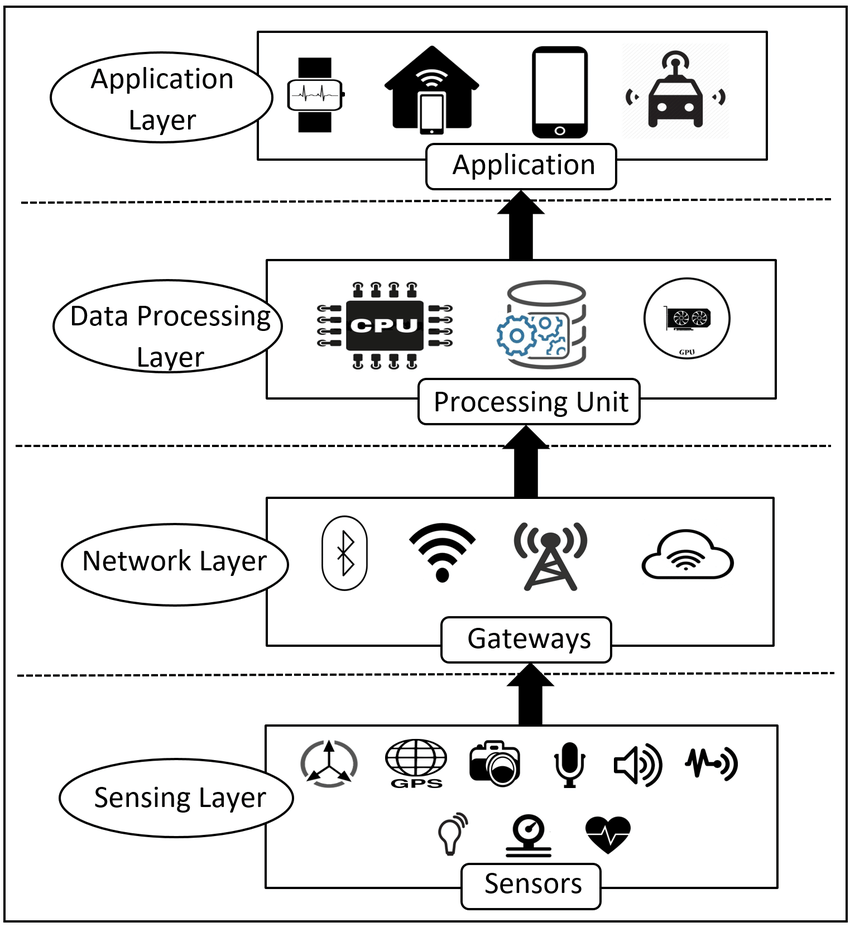
\includegraphics[width=0.7\linewidth]{figures/IoT-Architecture-Layers-and-Components.png}
%  \caption{Diagrama general de un sistema IoT}
%  \label{fig:IoT_General}
%\end{figure}


\section{Contexto tecnológico}

    En esta sección se describirán las tecnologías y herramientas más relevantes que se utilizarán a lo
    largo del desarrollo proyecto. El uso de las mismas se describirá en la sección \ref{chapter:desarrollo}.
    \todo{referenciar seccion correspondiente}

    \subsection{Gestión del proyecto}
        \subsubsection{Notion}
        \subsubsection{Microsoft Teams}
        \subsubsection{Zotero}
        \subsubsection{\LaTeX y Overleaf}
        

    \subsection{Ingeniería del Software}
        \subsubsection{Inyección de dependencias}
        \subsubsection{Integración continua}
        \subsubsection{Control de versiones}

    \subsection{Aplicación móvil}

        \subsubsection{Android}

            A grandes rasgos, Android es un Sistema Operativo orientado a dispositivos móviles basado en el núcleo 
            Linux, diseñado para ser independente de la arquitectura hardware de dichos dispositivos. 
            Si bien originalmente fue planteado para teléfonos móviles, con el avance de la industria ha adopado 
            un enfoque más amplio y es compatible con más dispositivos: tabletas, relojes inteligentes, televisores, 
            pantallas de automóviles... aunque, excepto en el caso de las tabletas, se trata de versiones basadas en
            Android con su propia idionsincrasia. \newline

            \begin{figure}[h]
                \centering
                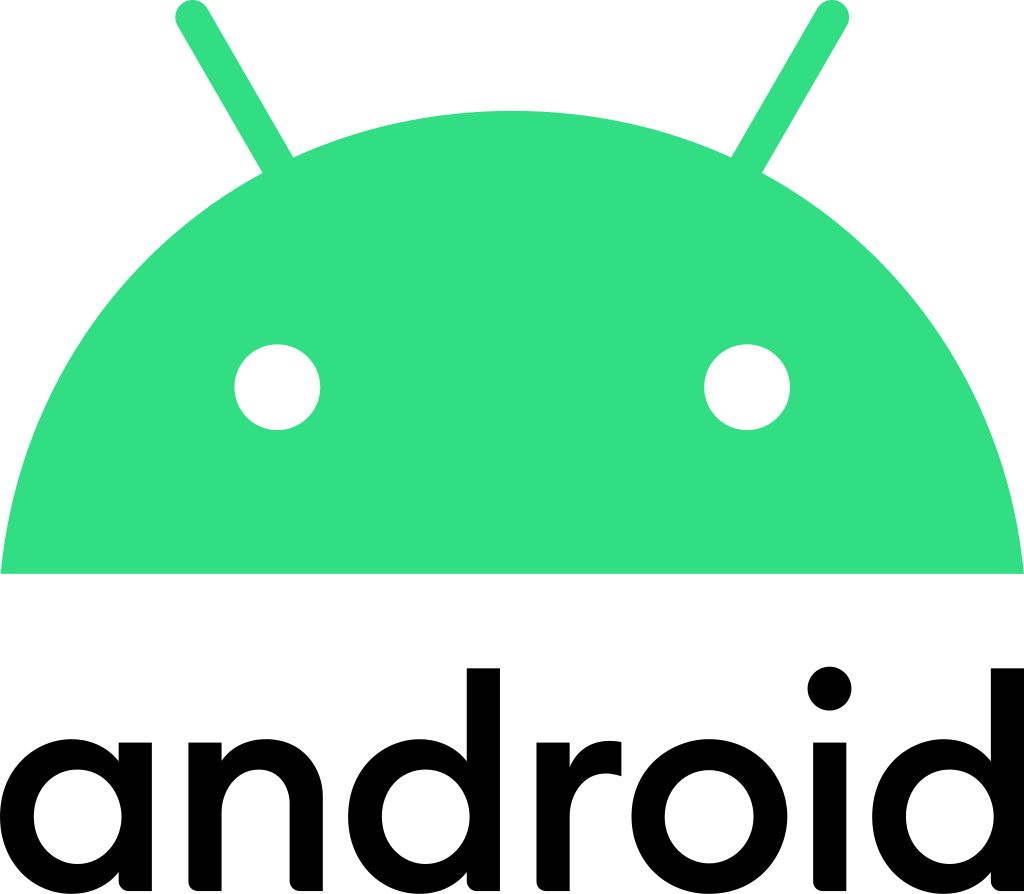
\includegraphics[width=0.25\textwidth]{figures/Android logo.png}
                \caption[Logo actual de Android.]
                {Logo actual de Android. Imagen extraída de \cite{vulcansphere_english_2019}}
                \label{figure:android:logo}
            \end{figure}

            Normalmente cuando nos referimos a Android, no nos referimos únicamente al sistema operativo, sino a la
            plataforma creada entorno al mismo; como haremos a lo largo de este proyecto. Dicha plataforma o 
            \textit{framework} consta de numerosas capas, siendo el sistema operativo una parte de ellas. El sistema 
            operativo como tal es denominado AOSP o \textit{Android Open Source Project}, siendo su código fuente 
            público. Cualquier persona puede acceder a él, descargarlo y modificiarlo \cite{collado_que_2022}.

            \begin{figure}[h]
                \centering
                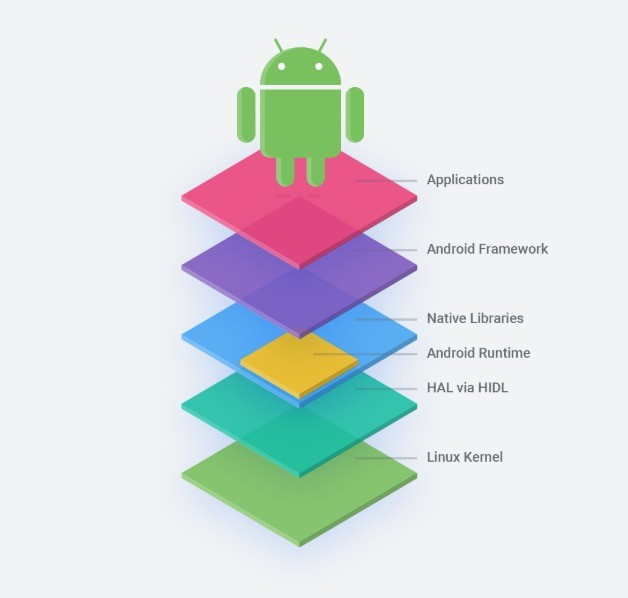
\includegraphics[width=0.66\textwidth]{figures/Android capas.jpg}
                \caption[Capas de Android.]
                {Capas de Android. Imagen extraída de \cite{perez_aosp_2019}}
                \label{figure:android:capas}
            \end{figure}

            No obstante, en la inmensa mayoría de los teléfonos móviles el sistema operativo es complementado con,
            entre otros, los GMS (\textit{Google Mobile Services}, o servicios de Google), los cuales solo están 
            disponibles bajo licencia; otorgada a los fabricantes que cumplen con una serie de requisitos. Los GMS 
            se utilizan para tareas como la gestión de notificaciones, servicios de geolocalización... además de para 
            acceder a las herramientas de Google, como la tienda de aplicaciones Play Store. Los fabricantes también 
            pueden personalizar y añadir funciones al sistema operativo, lo que explica que dos terminales con la misma 
            versión puedan verse tan diferentes entre sí. \newline

            Por otra parte, Android fue inicialmente desarrollado por la empresa homónima, si bien fue comprada en 2005
            por Google por 50 millones de dólares. La salida del sistema operativo se produciría dos años después, el 5 
            de noviembre de 2007, si bien el primer terminal que lo utilizaba (HTC Dream, también conocido como 
            T-Mobile G1) fue comercializado el 23 de septiembre de 2008 \cite{adeva_android_2023} \cite{marquez_asi_2022}.

            \begin{figure}[h]
                \centering
                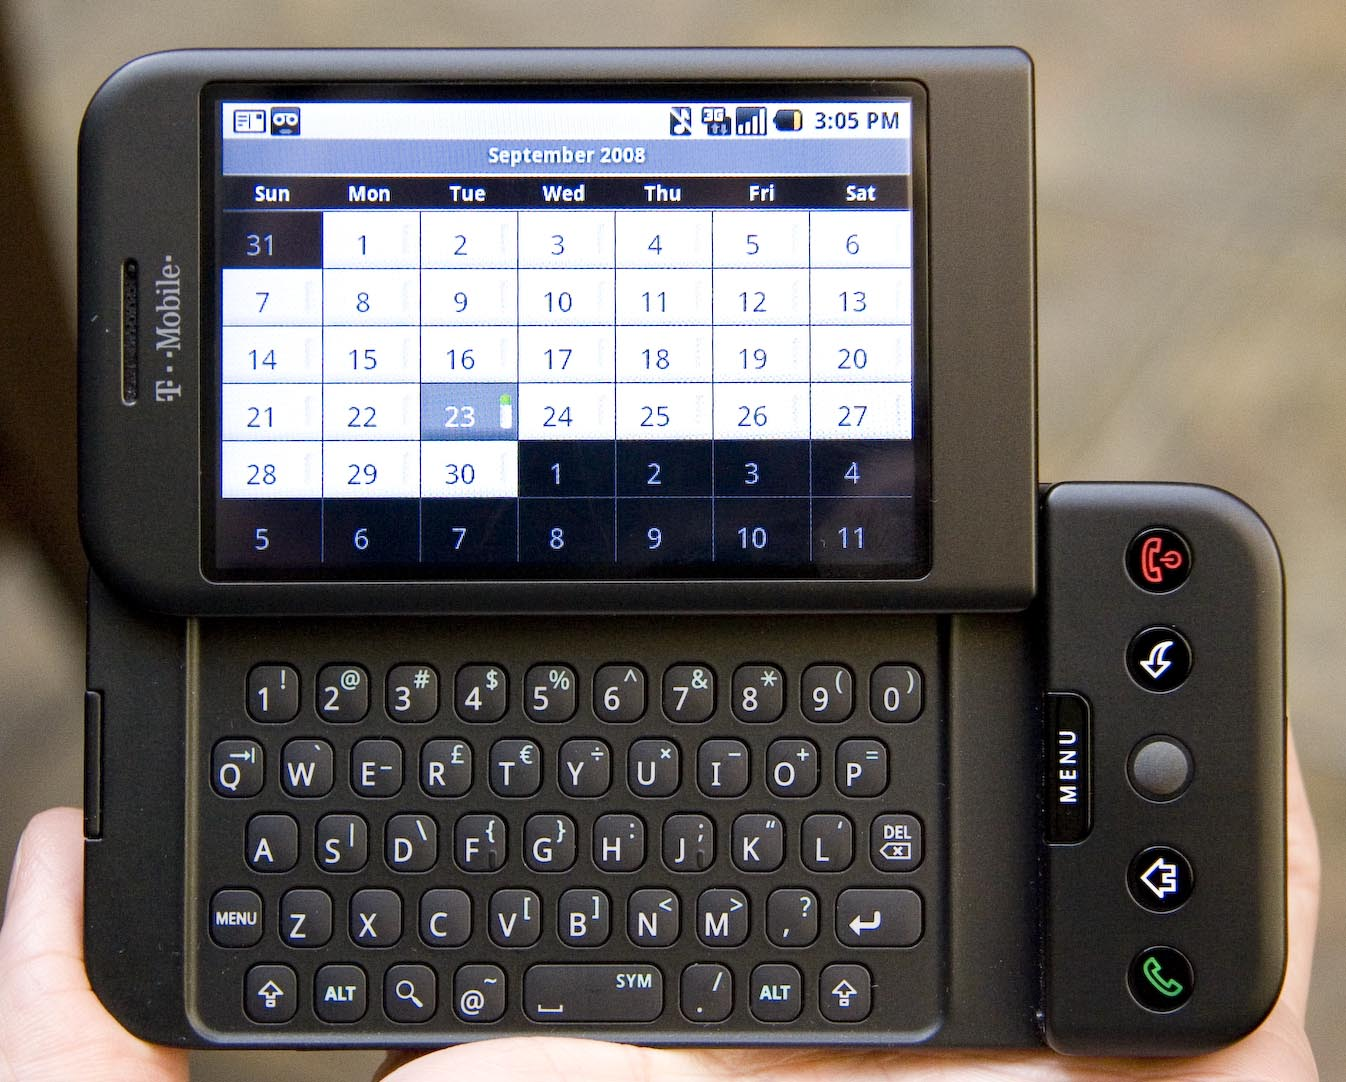
\includegraphics[width=0.5\textwidth]{figures/HTC Dream.jpg}
                \caption[HTC Dream en funcionamiento.]{HTC Dream en funcionamiento. Imagen extraída de \cite{oryl_t-mobile_2008}}
                \label{figure:android:htc_dream}
            \end{figure}

            Desde entonces, numerosas versiones de Android han sido lanzadas, siendo la última versión estable Android 
            13; estableciéndose por parte de Google la \textit{costumbre} de lanzar cada año una nueva versión principal. 
            En cada una de ellas se introducen nuevas características, pero esto no significa que todos los dispositivos 
            puedan actualizar. Los fabricantes no están obligados a actualizar sus terminales, lo que en la práctica 
            supone que las nuevas versiones no son utilizadas masivamente y que los programadores deben de tener en 
            cuenta las versiones antiguas en sus aplicaciones. 
            \newline

            Debido a que Google dejó de publicar oficialmente las estadísticas de uso de su sistema operativo, no es
            posible conocer con plena exactitud dichas cifras. La comunidad se ha encargado de estimar dicha 
            información \cite{belinski_android_nodate}; relevando que a fecha de mayo de 2023 sólo el 20\% de los 
            dispositivos tienen la última versión, mientras que las versiones 12,11 y 10 están presentes en el 
            20,8\%, 21,1\% y 16,6\% respectivamente. \newline

            \begin{figure}[H]
                \centering
                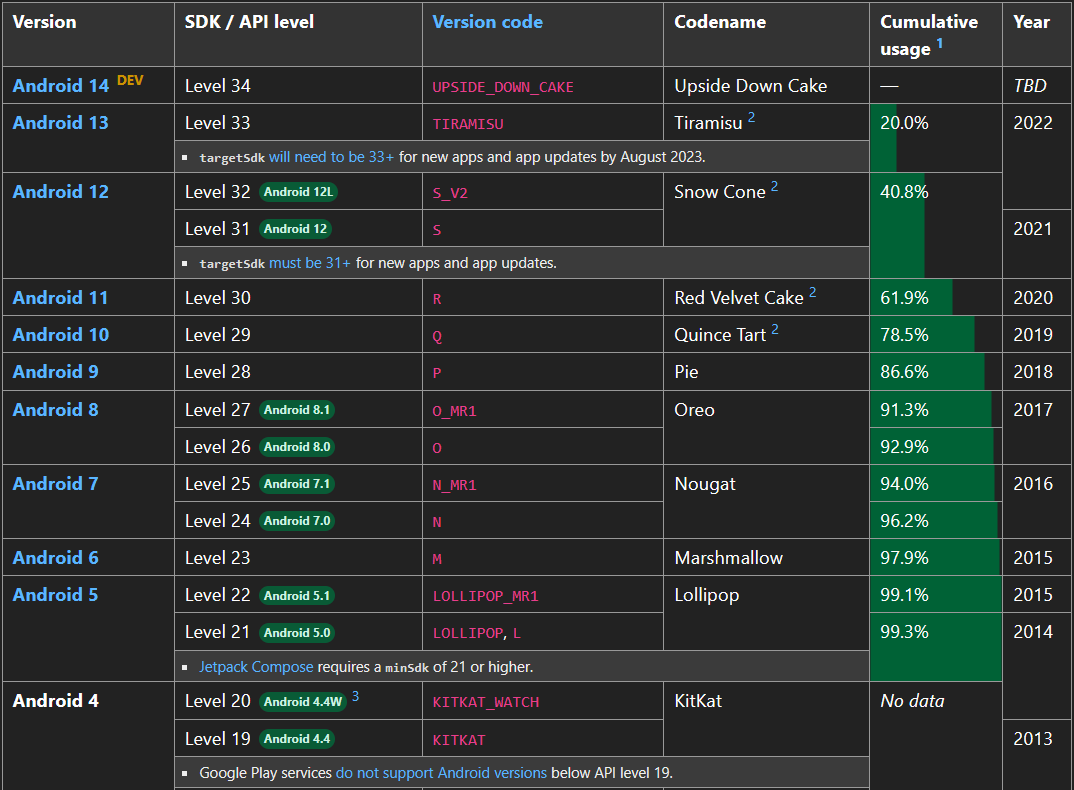
\includegraphics[width=1\textwidth]{figures/Android usage.PNG}
                \caption[Estadísiticas acumulativas de las versiones de Android]
                {Estadísiticas acumulativas de las versiones de Android. Imagen extraída de \cite{belinski_android_nodate}}
                \label{figure:android:usage}
            \end{figure}

            Por último, a fecha de marzo de 2023, Android dispone de una cuota de mercado del 71\% en el segmento de sistemas 
            operativos para dispositivos móviles, teniendo su mayor rival,el sistema operativo iOS (propiedad de Apple) 
            un 28\%. Entre ambos acaparan el mercado, con un 99\% de cuota de mercado. En cuanto a España, el 
            porcentaje de Android asciende hasta el 77,73\% por el 21,81 de iOS \cite{press_asi_2023}.

        \subsubsection{Kotlin}
            Durante el diseño de Android se estableció que el lenguaje principal para desarrollar aplicaciones sería 
            Java, si bien incorpora soporte para utilizar código C y C++ \cite{android_developers_como_nodate}. No
            obstante, al ser Java un lenguaje interpretrado sobre una máquina virtual (JVM o \textit{Java Virtual
            Machine}) se abrió la puerta para que se pudieran utilizar otros lenguajes basados que usasen la JVM, como
            ocurriría eventualmente con Kotlin.

        \subsubsection{Jetpack Compose}

        \subsubsection{Material Design 3}

        \subsubsection{Salud Conectada}

        \subsubsection{Room}

    
    \subsection{Servidor}
        \subsubsection{Python}

        \subsubsection{Flask}

        \subsubsection{MongoDB}
